\documentclass[margin=0mm]{standalone}

%% Language, Fonts, Encoding
\usepackage[english]{babel}                         % Input encoding language
\usepackage{fontspec}                               % XeTeX font settingss
\defaultfontfeatures{Ligatures=TeX, Numbers=Lining} % OTF font features for all fonts 
\setmainfont{Linux Libertine O}                     % Set serif (main) font 
\setsansfont{Linux Biolinum O}                      % Set sans serif font
\setmonofont{Inconsolata}                           % Set monospace font
\usepackage{amsmath, amssymb}                       % Math support
\newcommand{\mathbff}[1]{$\boldsymbol{#1}$}

\usepackage{tikz}                                        % Support for vector graphics
\usepackage{caption}                                     % Support for cpations inside tikz
% \usepackage{capt-of}                                     % Support for captions outside tikz
\usepackage{calc}                                        % Support for coordinate operations in tikz
\usepackage[nooldvoltagedirection, european]{circuitikz} % Support for electric circuit diagrams
\def \circuitsscale{0.6}                                 % Default value for circuit scale in this document

%% Circuit macros
\newcommand{\opampPMCenter}[1]{($(#1.+)!0.5!(#1.-)$) coordinate(opampPMCenter-PM) ($(#1.center) - (opampPMCenter-PM)$)  coordinate(opampPMCenter)} % Opamp center macro

\begin{document}
    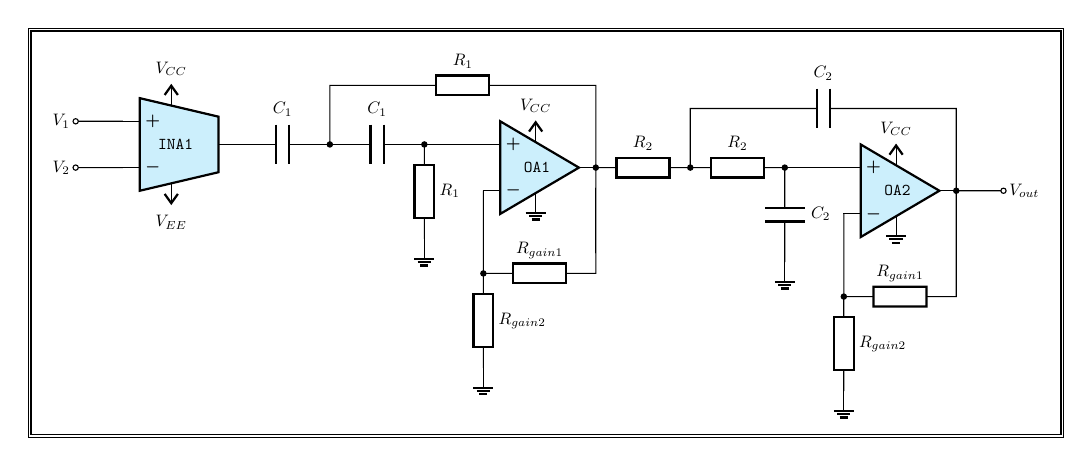
\begin{tikzpicture}[baseline={(current bounding box.center)}]
        \node{    
            \begin{circuitikz}[scale=\circuitsscale, transform shape, use fpu reciprocal]
                \draw (0,0)
                    node[inst amp, noinv input up, fill=cyan!20](INA1){\texttt{INA1}}
                    \opampPMCenter{INA1};
                \draw (INA1.+) ++(-1,0)
                    node[left]{$V_1$}
                    to[short, o-] ++(1,0);
                \draw (INA1.-) ++(-1,0)
                    node[left]{$V_2$}
                    to[short, o-] ++(1,0);
                \draw (INA1.up)
                    node[vcc]{$V_{CC}$};
                \draw (INA1.down)
                    node[vee]{$V_{EE}$};

                \draw (INA1.out)
                    to[C, l=$C_1$, -*] ++(2,0)
                    coordinate(C1-1)
                    to[C, l=$C_1$, -*] ++(2,0)
                    coordinate(C1-2);
                \draw (C1-2)
                    -- ++(1.25,0)
                    node[op amp, noinv input up, fill=cyan!20, anchor=+](OA1){\texttt{OA1}};
                \draw (C1-2)
                    to[R, l=$R_1$] ++(0,-2)
                    node[ground]{};
                \draw (OA1.-)
                    -- ++(0,-1.75)
                    coordinate(Rg1Rg2)
                    to[R, l=$R_{gain1}$, *-] (Rg1Rg2-|OA1.out)
                    to[short, -*] (OA1.out);
                \draw (Rg1Rg2)
                    to[R, l=$R_{gain2}$] ++(0,-2)
                    node[ground]{};
                \draw (C1-1)
                    -- ++(0,1.25)
                    coordinate(R1-1start)
                    to[R, l=$R_1$] (R1-1start-|OA1.out)
                    -- (OA1.out);
                \draw (OA1.up)
                    node[vcc]{$V_{CC}$};
                \draw (OA1.down)
                    node[ground]{};
                
                \draw (OA1.out)
                    to[R, l=$R_2$, -*] ++(2,0)
                    coordinate(R2-1)
                    to[R, l=$R_2$, -*] ++(2,0)
                    coordinate(R2-2);
                \draw (R2-2)
                    -- ++(1.25,0)
                    node[op amp, noinv input up, fill=cyan!20, anchor=+](OA2){\texttt{OA2}};
                \draw (R2-2)
                    to[C, l=$C_2$] ++(0,-2)
                    node[ground]{};
                \draw (OA2.-)
                    -- ++(0,-1.75)
                    coordinate(Rg1Rg2)
                    to[R, l=$R_{gain1}$, *-] (Rg1Rg2-|OA2.out)
                    to[short, -*] (OA2.out);
                \draw (Rg1Rg2)
                    to[R, l=$R_{gain2}$] ++(0,-2)
                    node[ground]{};
                \draw (R2-1)
                    -- ++(0,1.25)
                    coordinate(C2-1start)
                    to[C, l=$C_2$] (C2-1start-|OA2.out)
                    -- (OA2.out);
                \draw (OA2.out) ++(1,0)
                    node[right]{$V_{out}$}
                    to[short, o-] ++(-1,0);
                \draw (OA2.up)
                    node[vcc]{$V_{CC}$};
                \draw (OA2.down)
                    node[ground]{};
                    
            \end{circuitikz}
            };

        \draw[black, double]
            (current bounding box.south west) ++(-\fboxsep, -\fboxsep) coordinate (ll)
            (current bounding box.north east) ++(\fboxsep, \fboxsep) coordinate (ur)
            (ll) rectangle (ur);
    \end{tikzpicture}
\end{document}